% !TEX TS-program = XeLaTeX

% STYLE

\documentclass[a4paper, 12pt]{article}
\usepackage[left=1in,
		    right=1in,
    		    top=1in,
		    bottom=1in,
		    bindingoffset=0cm]{geometry}
		    \usepackage{array}
\usepackage{float}
\usepackage{graphicx}
\graphicspath{ {./images/} }
\usepackage{subfig}
\usepackage{enumerate}
\usepackage[normalem]{ulem} % underlining
\usepackage{booktabs} % tables
\usepackage[table]{xcolor} % coloring tables
\newcolumntype{L}[1]{>{\raggedright\let\newline\\\arraybackslash\hspace{0pt}}m{#1}} % beautiful column types
\newcolumntype{C}[1]{>{\centering\let\newline\\\arraybackslash\hspace{0pt}}m{#1}}

% LANGUAGE + FONT
		    
\usepackage[english]{babel}
\usepackage[backend=biber,
                     style=unified]{biblatex}
\newcommand{\citeay}[2][]{
   \citeauthor{#2} (\citeyear[#1]{#2})}
\addbibresource{ref.bib}
\usepackage{fontspec}  
\setmainfont{Minion 3}

% DRAWING

\usepackage{tikz}
\usepackage{tikz-qtree}
\usetikzlibrary{shapes.geometric}
\usetikzlibrary{trees,arrows}
\usetikzlibrary{positioning}
\usetikzlibrary{matrix}
\usetikzlibrary{tikzmark}
\usetikzlibrary{decorations.shapes}

% LINGUISTICS 

\usepackage{expex}
\usepackage[glossaries]{leipzig}
\makeglossaries
\newleipzig {npst} {npst} {non-past}
\newleipzig {nfin} {nfin} {non-finite}
\newleipzig {nsg} {nsg} {non-singular}

\lingset{numoffset=1ex, aboveexskip=1em, belowexskip=1em}

\title{Kazym Khanty schwa}
\author{Sasha Shikunova, EGG2023, Novi Sad}
\date{Last updated \today}

\begin{document}
\maketitle

	\section{Basic facts}
	
	Russia, Khanty-Mansi autonomous region, Kazym
	
	\begin{figure}[H]
		\centering
		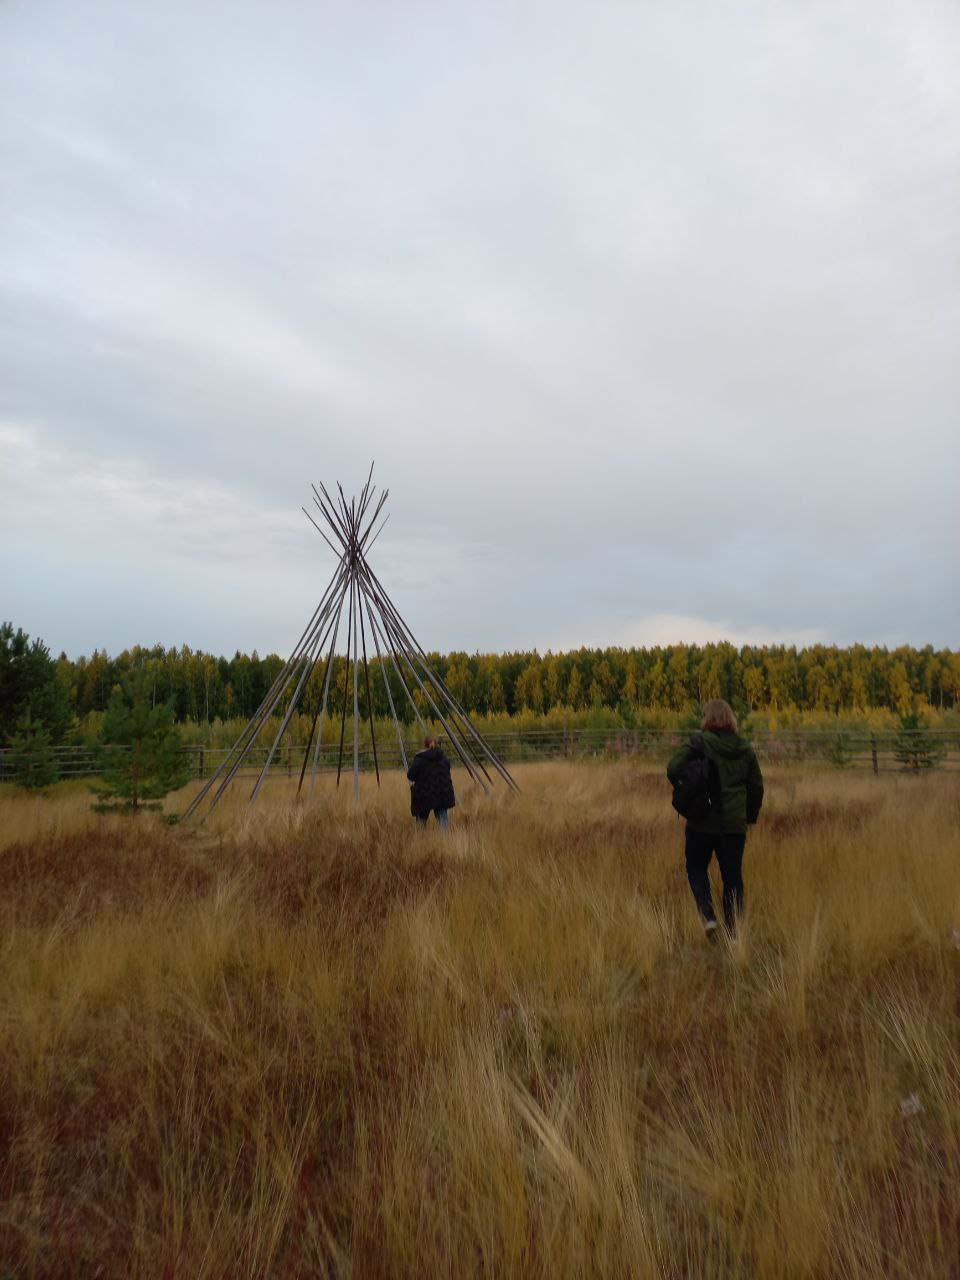
\includegraphics[scale=.167]{beginning}
		\hfill
		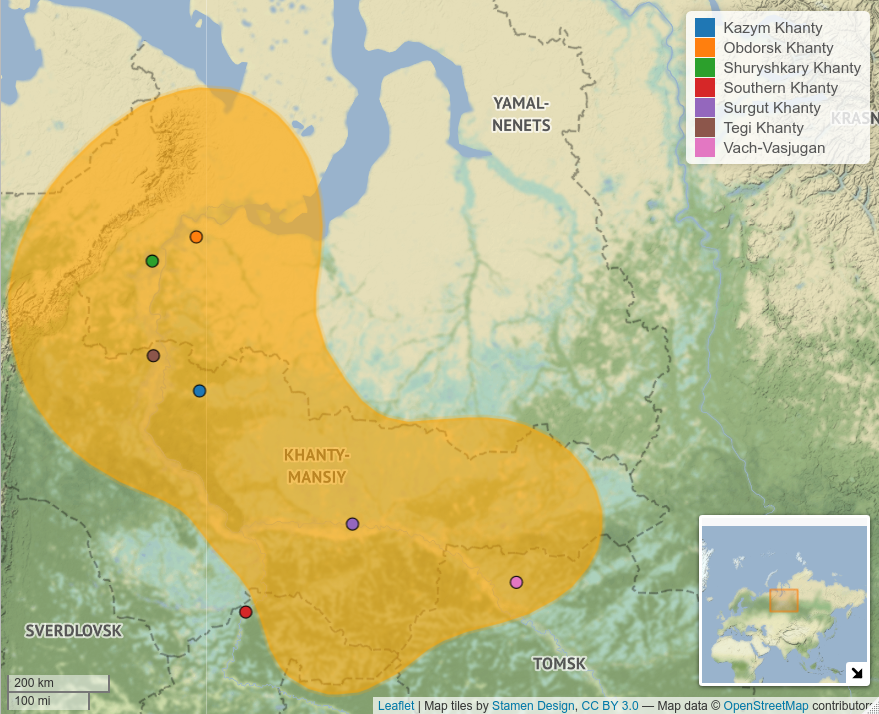
\includegraphics[scale=.4]{map}
	\end{figure}

	\noindent Vowel and consonant inventories \parencite{lketal2018}. In the practical transcription, λ = ɬ
	
	\begin{figure}[H]
		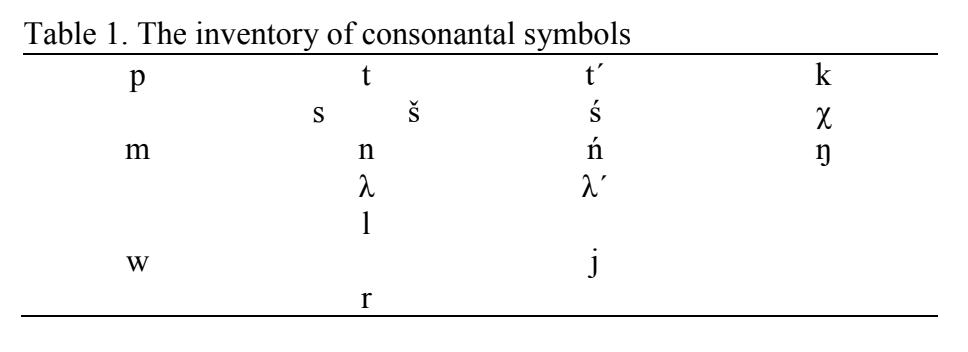
\includegraphics[scale=.66]{consonants}
	\end{figure}
	
	\newpage
	\noindent Not every vowel occurs in the first syllable:
	
	\begin{figure}[H]
		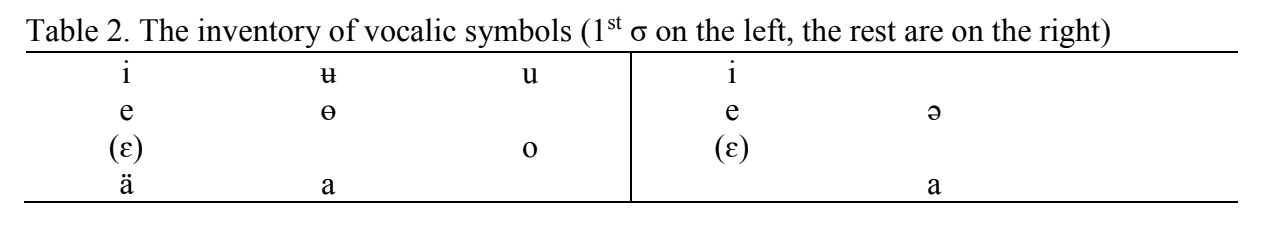
\includegraphics[scale=.66]{vowels}
	\end{figure}
	
\begin{enumerate}[$\gg$]
	\item No contrastive voicing
	\item Less vowel quality contrast in non-initial syllables (in native Khanty words; cf. \emph{kǎrtɵpka} `potato' -- Russian loanword)
\end{enumerate}
	Nominal inflection:

\begin{enumerate}[$\gg$]
	\item base - number - possessive - case (\ref{ex:nouninfl})
	\item if the base ends in /u i/, insertion of /w j/ is possible with some morphemes (\emph{wʉλi} + \emph{(ə)n} $\rightarrow$ \emph{wʉλijn} `deer-{\Loc}')
\end{enumerate}

\ex
\begingl\label{ex:nouninfl}
	\gla jaj-λ-aλ-a//
	\glb brother-{\Pl}-{\Poss}.{\Tsg}-{\Dat}//
	\glft `{\Tsg}'s brother'//
\endgl
\xe
	Verbal inflection:

\begin{enumerate}[$\gg$]
	\item base - tense - inversive - agreement (\ref{ex:verbinfl})
	\item if the base ends in /u i/, insertion of /w j/ sometimes occurs (\emph{ari + (ə)s} $\rightarrow$ \emph{ari-js} `sing-{\Pst}')
	\item infinitive: base + \emph{ti/əm} ({\Npst}/{\Pst}); \emph{əm} after /u i/ causes insertion of /w j/ (\emph{tɵ-ti} `carry-{\Nfin}.{\Npst}' vs \emph{tʉw-əm} `carry-{\Nfin}.{\Pst}')
\end{enumerate}

\pex
\a\begingl\label{ex:verbinfl}
	\gla λɵt-s-aj-ən//
	\glb buy-{\Pst}-{\Pass}-{\Ssg}//
	\glft `you were bought'//
\endgl
\xe

	\section{Vowel-zero alternations}

	Schwa is a phoneme, see a minimal pair in (\ref{ex:minpair}). 
	
\pex\label{ex:minpair}
\a \emph{kurt} `iron'
\a \emph{kur-ət} `bull-{\Pl}'
\xe
	
	\noindent 3 types of verbal bases wrt. schwa behaviour:
	
\begin{table}[H]
\centering
\begin{tabular}{l c c c}
\toprule
\textbf{Form}
&
\textbf{No schwa}
&
\textbf{Alternating schwa}
&
\textbf{Stable schwa}
\\
\midrule
& 	ort- `divide' &		ir(ə)t- `turn' &		orət- `drag'\\
\addlinespace[0.2cm]
{\Npst}{[{\Tsg}]}& 	ort-əλ $\sim$ orλ &		irət-λ&		orət-λ\\
\addlinespace[0.2cm]
{\Pst}{[{\Tsg}]}&ort-əs&		irt-əs&orət-s		\\
\addlinespace[0.2cm]
{\Npst}-{\Ssg}&or-λ-ən&	irt-λ-ən	&	orət-λ-ən	\\
\addlinespace[0.2cm]
{\Pst}-{\Ssg}&or-s-ən&		irt-s-ən&	orət-s-ən	\\
\addlinespace[0.2cm]
{\Npst}-{\Fdu}&or-λ-əmn&	irt-λ-əmn	&	orət-λ-əmn	\\
\addlinespace[0.2cm]
{\Pst}-{\Fdu}&or-s-əmn&		irt-s-əmn&	orət-s-əmn	\\
\bottomrule
\end{tabular}
\label{t:verbpar}
\end{table}

	\noindent Vowel-final verb bases:

\ex Ca\#\\
\emph{χunta-s} `run-{\Pst}' --- \emph{χunta-s-n} `run-{\Pst}-{\Ssg}'
\xe

\ex Ci\#\\
\emph{arij-s} `sing-{\Pst}' --- \emph{ari-s-ən} `sing-{\Pst}-{\Ssg}'
\xe

\ex Cə\#\\
\emph{pɵrλə-s} `soar-{\Pst}' --- \emph{pɵrλə-s-n} `soar-{\Pst}-{\Ssg}'\\
also: \emph{pɵrλə-s-mən} `soar-{\Pst}-{\Fdu}'
\xe

	\pex[nopreamble=true] \label{ex:problem}
	\a {ari + əs} $\rightarrow$ {arijəs} $\rightarrow$ {arijs}
	\a {ari + əs + ən} $\rightarrow$ {ari + s + ən} \hfill \parencite{egorov2022}
	\xe
	
	\noindent Nominal inflection: possessive vs case markers
	
\begin{table}[H]
\centering
\begin{tabular}{l c c c}
\toprule
\textbf{Form}
&
\textbf{Ci\#}
&
\textbf{Ca\#}
&
\textbf{CVC\#}
\\
\midrule
& 	wʉλi `deer'&		λapka `shop'&		sʉmət (sʉmt) `birch'\\
\addlinespace[0.2cm]
{\Nom}& 	wʉλi&		λapka&		sʉmət (sʉmt)\\
\addlinespace[0.2cm]
{\Loc}&wʉλi-j(ə)n&		λapka-j(ə)n&sʉmət-n		\\
\addlinespace[0.2cm]
{\Poss}.{\Spl}&wʉλen&	λapka-j(ə)n	&	sʉmt-ən	\\
\bottomrule
\end{tabular}
\label{t:nompar}
\end{table}

	\section{Stress}
	
	Trochee with some quirks \parencite{tyutyunnikova2022}.
	
	\pex
	\a ˌpăsaˈnɛma \hfill păsan-ɛm-a `table-{\Poss}.{\Fsg}-{\Dat}'
	\a ˈλaraś \hfill λaraś `box'
	\a ˈλaraˈśɛma \hfill λaraś-ɛm-a `box-{\Poss}.{\Fsg}-{\Dat}'
	\a ˈλaraśa \hfill λaraś-a `box-{\Dat}'
	\a ˈpăsan \hfill păsan `table'
%	\a λaˈraś(ə)λa \hfill λaraś-(ə)λ-a `box-{\Poss}.{\Tsg}-{\Dat}'
	\a ˌmuχəˈλaja \hfill muχəλaja `around'
	\a ˌjuntˈλaλən \hfill junt-λ-aλ-ən `game-{\Pl}-{\Poss}.{\Tsg}-{\Loc}'
	\xe
	
	\noindent Interaction with schwa \parencite{tyutyunnikova2023}.
	
	\pex
	\a λaˈraśλa \hfill λaraś-(ə)λ-a `box-{\Poss}.{\Tsg}-{\Dat}'
	\a ˈpaknəλˈsəmn \hfill paknəλ-(ə)s-əm(ə)n `scare-{\Pst}-{\Tdu}'
	\a ˈpirśˈλaλən \hfill pir(ə)ś-λ-aλ-ən `old-{\Pl}-{\Poss}.{\Tsg}-{\Loc}'
	\a kɵrˈtəta $\sim$ ˈkɵrtəta \hfill kɵrt-ət-a `settlement-{\Pl}-{\Dat}'
	\a ˈsewrsaˈλəmn \hfill sew(ə)r-(ə)s-aλəm(ə)n `chop-{\Pst}-{\Fdu}>{\Nsg}'
	\xe
	
	\section{Summary of observations}

	Schwa is not always epenthetic:
	
\begin{enumerate}[$\gg$]
	\item There is a minimal pair where schwa makes the difference
	\item Schwa in the suffix can cause glide epenthesis -- sign of an underlying rather than an epenthetic vowel
\end{enumerate}
	Verbal bases with schwa can be divided into 2 classes:
	
\begin{enumerate}[$\gg$]
	\item Stable non-alternating schwa (\emph{orət-} `to drag')
	\item Alternating schwa (\emph{ir(ə)t-} `to turn')
\end{enumerate}
	In the verbal agreement suffix \emph{-əmən} `{\Fdu}' either of the two schwas can be present, depending on whether the base ends in a vowel or a consonant:
	
	\pex Schwa alternation in \emph{-əmən} `{\Fdu}'
		\a \emph{irt-s-əmn} `turn-{\Pst}-{\Fdu}' \hfill C\#
		\a \emph{orət-s-əmn} `drag-{\Pst}-{\Fdu}' \hfill C\#
		\a \emph{ji-s-mən} `become-{\Pst}-{\Fdu}' \hfill V\#
	\xe
	The schwa in the {\Ssg} suffix \emph{-ən} can disappear in the same circumstances as the initial schwa of \emph{-əmən} `{\Fdu}'.
	
	\pex Schwa alternation in \emph{-ən} `{\Ssg}'
		\a \emph{irt-s-ən} `turn-{\Pst}-{\Fdu}' \hfill C\#
		\a \emph{orət-s-ən} `drag-{\Pst}-{\Fdu}' \hfill C\#
		\a \emph{xunta-s-n} `run-{\Pst}-{\Fdu}' \hfill V\#
	\xe
	There is occasional glide insertion after /i/-final bases, which can be conditioned by the presence of overt agreement morphology after the tense marker:
	
\ex\emph{arij-s} `sing-{\Pst}' --- \emph{ari-s-ən} `sing-{\Pst}-{\Ssg}'
\xe
	In the nominal paradigm, there is glide insertion before some suffixes (\ref{loc}) and vowel coalescence before others (\ref{poss}).
	
	\ex\label{loc}\emph{wʉλi} + \emph{ən} $\rightarrow$ \emph{wʉλij(ə)n} `deer-{\Loc}' \xe
	\ex~\label{poss}\emph{wʉλi} + \emph{ən} $\rightarrow$ \emph{wʉλen} `deer-{\Poss}.{\Spl}' \xe
	

	\section*{Glossing abbreviations}
	
\printglossaries
	
\printbibliography

	\begin{figure}[H]
		\centering
		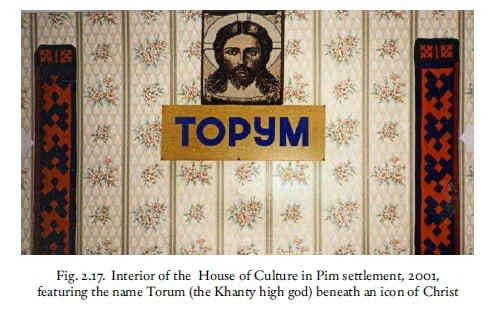
\includegraphics[scale=.66]{end}
	\end{figure}

\end{document}